\documentclass[a4paper,twoside]{article}
\usepackage{blindtext}  
\usepackage{geometry}

% Chinese support
\usepackage[UTF8, scheme = plain]{ctex}

% Page margin layout
\geometry{left=2.3cm,right=2cm,top=2.5cm,bottom=2.0cm}


\usepackage{listings}
\usepackage{xcolor}
\usepackage{geometry}
\usepackage{amsmath}
\usepackage{float}
\usepackage{hyperref}

\usepackage{graphics}
\usepackage{graphicx}
\usepackage{subfigure}
\usepackage{epsfig}
\usepackage{float}

\usepackage{algorithm}
\usepackage[noend]{algpseudocode}

\usepackage{booktabs}
\usepackage{threeparttable}
\usepackage{longtable}
\usepackage{listings}
\usepackage{tikz}

% cite package, to clean up citations in the main text. Do not remove.
\usepackage{cite}

\usepackage{color,xcolor}

%% The amssymb package provides various useful mathematical symbols
\usepackage{amssymb}
%% The amsthm package provides extended theorem environments
\usepackage{amsthm}
\usepackage{amsfonts}
\usepackage{enumerate}
\usepackage{enumitem}
\usepackage{listings}

\usepackage{indentfirst}
\setlength{\parindent}{2em} % Make two letter space in the first paragraph
\usepackage{setspace}
\linespread{1.5} % Line spacing setting
\usepackage{siunitx}
\setlength{\parskip}{0.5em} % Paragraph spacing setting

% \usepackage[contents =22920202204622, scale = 10, color = black, angle = 50, opacity = .10]{background}

\newcommand*{\dif}{\mathop{}\!\mathrm{d}}

\renewcommand{\figurename}{图}
\renewcommand{\lstlistingname}{代码} 
\renewcommand{\tablename}{表格}
\renewcommand{\contentsname}{目录}
\floatname{algorithm}{算法}

\graphicspath{ {images/} }

%%%%%%%%%%%%%
\newcommand{\StudentNumber}{22920202204622}  % Fill your student number here
\newcommand{\StudentName}{熊恪峥}  % Replace your name here
\newcommand{\PaperTitle}{实验(三)\ \ 实现龙贝格积分}  % Change your paper title here
\newcommand{\PaperType}{计算方法(A)} % Replace the type of your report here
\newcommand{\Date}{2022年4月6日}
\newcommand{\College}{信息学院}
\newcommand{\CourseName}{计算方法(A)}
%%%%%%%%%%%%%

%% Page header and footer setting
\usepackage{fancyhdr}
\usepackage{lastpage}
\pagestyle{fancy}
\fancyhf{}
% This requires the document to be twoside
\fancyhead[LO]{\texttt{\StudentName }}
\fancyhead[LE]{\texttt{\StudentNumber}}
\fancyhead[C]{\texttt{\PaperTitle }}
\fancyhead[R]{\texttt{第{\thepage}页,共\pageref*{LastPage}页}}


\title{\PaperTitle}
\author{\StudentName}
\date{\Date}

\lstset{
	basicstyle          =   \sffamily,          % 基本代码风格
	keywordstyle        =   \bfseries,          % 关键字风格
	commentstyle        =   \rmfamily\itshape,  % 注释的风格,斜体
	stringstyle         =   \ttfamily,  % 字符串风格
	flexiblecolumns,                % 别问为什么,加上这个
	numbers             =   left,   % 行号的位置在左边
	showspaces          =   false,  % 是否显示空格,显示了有点乱,所以不现实了
	numberstyle         =   \zihao{-5}\ttfamily,    % 行号的样式,小五号,tt等宽字体
	showstringspaces    =   false,
	captionpos          =   t,      % 这段代码的名字所呈现的位置,t指的是top上面
	frame               =   lrtb,   % 显示边框
}

\lstdefinestyle{PythonStyle}{
	language        =   Python, % 语言选Python
	basicstyle      =   \zihao{-5}\ttfamily,
	numberstyle     =   \zihao{-5}\ttfamily,
	keywordstyle    =   \color{blue},
	keywordstyle    =   [2] \color{teal},
	stringstyle     =   \color{magenta},
	commentstyle    =   \color{red}\ttfamily,
	breaklines      =   true,   % 自动换行,建议不要写太长的行
	columns         =   fixed,  % 如果不加这一句,字间距就不固定,很丑,必须加
	basewidth       =   0.5em,
}

\algnewcommand\algorithmicinput{\textbf{Input:}}
\algnewcommand\algorithmicoutput{\textbf{Output:}}
\algnewcommand\Input{\item[\algorithmicinput]}%
\algnewcommand\Output{\item[\algorithmicoutput]}%

\usetikzlibrary{positioning, shapes.geometric}

\begin{document}
	
%%%%%%%%%%%%%%%%%%%%%%%%%%%%%%%%%%%%%%%%%%%%
\makeatletter % change default title style
\renewcommand*\maketitle{%
	\begin{center} 
		\bfseries  % title 
		{\LARGE \@title \par}  % LARGE typesetting
		\vskip 1em  %  margin 1em
		{\global\let\author\@empty}  % no author information
		{\global\let\date\@empty}  % no date
		\thispagestyle{empty}   %  empty page style
	\end{center}%
	\setcounter{footnote}{0}%
}
\makeatother
%%%%%%%%%%%%%%%%%%%%%%%%%%%%%%%%%%%%%%%%%%%%
	
	
\thispagestyle{empty}

\vspace*{1cm}

\begin{figure}[h]
	\centering
	
\includegraphics[width=4.0cm]{logo.png}
\end{figure}

\vspace*{1cm}

\begin{center}
	\Huge{\textbf{\PaperType}}
	
	\Large{\PaperTitle}
\end{center}

\vspace*{1cm}

\begin{table}[h]
	\centering	
	\begin{Large}
		\renewcommand{\arraystretch}{1.5}
		\begin{tabular}{p{3cm} p{5cm}<{\centering}}
			姓\qquad 名 & \StudentName  \\
			\hline
			学\qquad号 & \StudentNumber \\
			\hline
			日\qquad期 & \Date  \\
			\hline
			学\qquad院 & \College  \\
			\hline
			课程名称 & \CourseName  \\
			\hline
		\end{tabular}
	\end{Large}
\end{table}

\newpage

\title{
	\Large{\textcolor{black}{\PaperTitle}}
}
	
	
\maketitle
	
\tableofcontents
 
\newpage
\setcounter{page}{1}

\begin{spacing}{1.2}

\section{实现}

龙贝格积分法是通过外推法不断使用梯形公式来提高计算精度的数值积分法。是一种常用的积分法,
并且可以达到较高的精度。

\subsection{文件结构}

本程序实现了龙贝格积分以及用于基准测试和比较的蒙特卡洛积分法和
拟蒙特卡洛(Quasi-Monte Carlo)积分法。主要文件和作用如表格~\ref{tbl:struct}所示。

\begin{table}[htbp]
	\centering
	\renewcommand\arraystretch{1.5}
	\begin{tabular}{p{4cm}p{6cm}}
		\toprule
		文件 & 作用 \\
		\midrule
		integral/romberg.py & 龙贝格积分实现 \\
		\hline
		integral/qmc.py & 拟蒙特卡洛积分法实现 \\
		\hline
		integral/montecarlo.py & 蒙特卡洛积分法实现 \\
		\bottomrule
	\end{tabular}
	\label{tbl:struct}
	\caption{主要文件和作用}
\end{table}

本程序依赖如下两个第三方库:
\begin{itemize}
	\item \textbf{Numpy}: 用于加速向量运算
	\item \textbf{Scipy}: 用于生成低差异序列(Low-discrepancy sequence)
\end{itemize}

\subsection{接口实现}

本程序为龙贝格积分法实现以下接口,它支持通过给定任意可调用对象(Callable)表示的函数进行积分,具有良好的可扩展性。
\begin{lstlisting}[language=Python,numbers=left,style=PythonStyle,label={code:interface}]
def integrate(f: Callable[[np.float], np.float], a: np.float, b: np.float, epsilon: np.float = 0.001,
              n: int = 32) -> np.float:
\end{lstlisting}

该接口有如下参数:
\begin{itemize}
	\item $\mathbf{f}$: 被积函数的可调用对象。
	\item $\mathbf{a}, \mathbf{b}$: 表示积分区间$[a,b]$。
	\item $\mathbf{epsilon}$: 当两次迭代数值变化$\Delta T\le \varepsilon$时停止迭代,可以控制积分精度。
	\item  $\mathbf{n}$: 最大迭代次数。
\end{itemize}


\section{基准测试}

\subsection{积分准确度和收敛速度}

为了测试龙贝格积分法的效果,以Matlab 2021b的积分值为真值、蒙特卡洛积分法和拟蒙特卡洛积分法为基线
进行测试,计算积分$\int_0^{\frac{\pi}{2}}\cos x \dif x$和$\int_0^4\sqrt[4]{15x^3+21x^2+41x+3}\cdot e^{-0.5x}\dif x$。被积函数
的图形如图~\ref{fig:funcs}

\begin{figure}[H]
	\centering 
	\subfigure[函数$f(x)=\cos x$]{ 
	  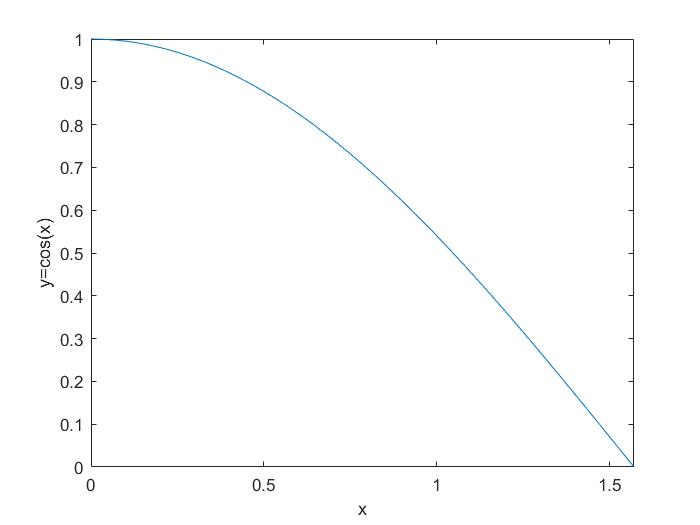
\includegraphics[width=0.48\textwidth]{func1.jpg} 
	} 
	~
	\subfigure[函数$g(x)=(15x^3+21x^2+41x+3)^{\frac{1}{4}}\cdot e^{-0.5x}$]{ 
	  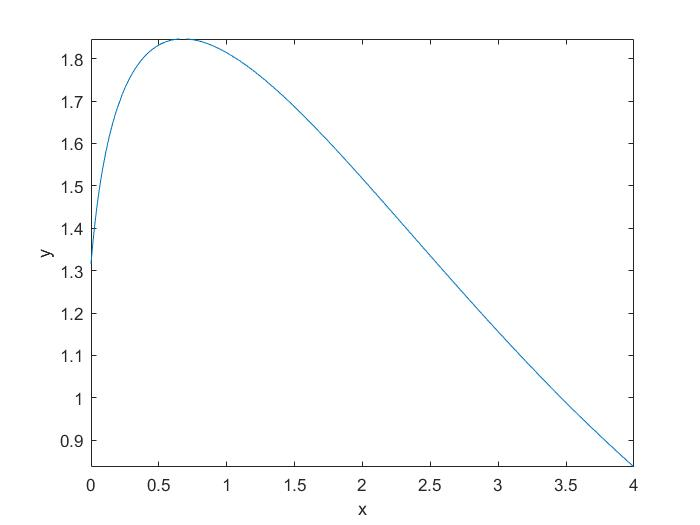
\includegraphics[width=0.48\textwidth]{func2.jpg} 
	} 
	\caption{被积函数图象} 
	\label{fig:funcs}
\end{figure}

调用本程序实现的龙贝格积分法函数,要求精度$0.0001$,迭代次数最多$128$次,可以得到每次迭代的
积分值如图~\ref{fig:converg}。可以发现龙贝格积分法的收敛速度很快,约3至4次迭代即可得到
和真实值相近的积分值。

\begin{figure}[H]
	\centering 
	\subfigure[积分$\int_0^{\frac{\pi}{2}}f(x)\dif x$迭代过程]{ 
	  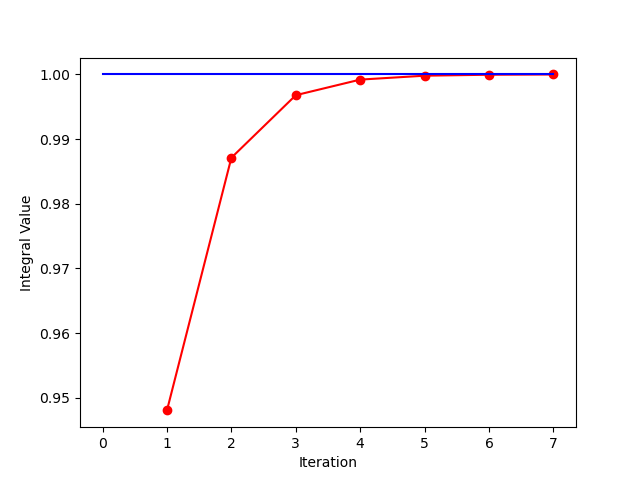
\includegraphics[width=0.48\textwidth]{convergence1.png} 
	} 
	~
	\subfigure[积分$\int_0^4g(x)\dif x$迭代过程]{ 
	  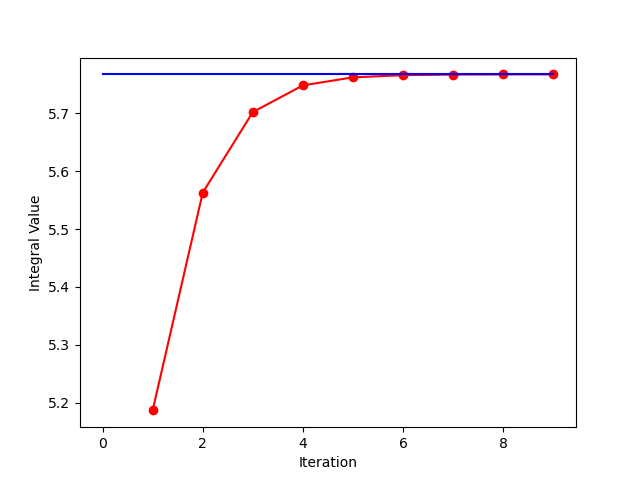
\includegraphics[width=0.48\textwidth]{convergence2.png} 
	} 
	\caption{被积函数图象} 
	\label{fig:converg}
\end{figure}

龙贝格积分法积分得出的数据如表~\ref{tbl:romberg}所示。在迭代次数$10$以内
的条件下积分值的精确度已经达到了极高的水平,相对误差对于两个不同的函数均小于$0.001\%$。
这说明了龙贝格法有良好的精度。

\begin{table}[htbp]
	\centering
	\begin{tabular}{cccc}
		\toprule
		函数 & 测量值 & 参考值(以Matlab 2021b为基准) & 相对误差(\%) \\
		\midrule
		$f(x)$ & $0.9999874501175262$ & $1$ & $0.0012$ \\
		$g(x)$ & $5.767412519408859$ & $5.767433490695931$ & $0.00036$ \\
		\bottomrule
	\end{tabular}
	\caption{龙贝格积分法积分值}
	\label{tbl:romberg}
\end{table}

\subsection{运行效率和比较}

平均运行时间用于测量该实现的运行效率,通过1000次循环取平均值来规避偶然波动。结果如
图~\ref{fig:rubtimeaverage}。可以发现龙贝格积分法的运行速度在函数本身不是非常复杂,
但是当函数求值较为复杂时,龙贝格积分法在效率上比其他两者较慢。其中的一个原因可能是
龙贝格法每轮迭代中函数求值发生的时间\emph{没有较强的时间上的局部性}。蒙特卡洛法
和拟蒙特卡洛法对函数求值会在采样点得出之后一次完成,而龙贝格法会在每轮迭代中
多次发生。

\begin{figure}[htbp]
	\centering
	\label{fig:rubtimeaverage}
	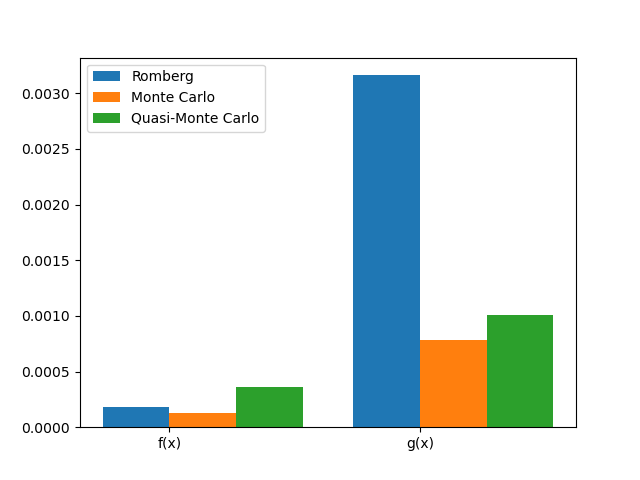
\includegraphics[width=0.5\linewidth]{runtime.png}
	\caption{平均运行时间}
\end{figure}

\subsection{蒙特卡洛和拟蒙特卡洛法的性能}

但是由于运行时间的差异实际上并不大,但这并不能否认龙贝格积分法是一个优秀的数值积分法。
因为龙贝格积分发可以给出一个确定的解,它在任何情况下多次调用都是稳定的。如图~\ref{fig:variance}
蒙特卡洛法具有一定的随机性,每次调用的值都分布在实际值附近,但是有所波动。

\begin{figure}[H]
	\centering 
	\subfigure[蒙特卡洛法500次分布]{ 
	  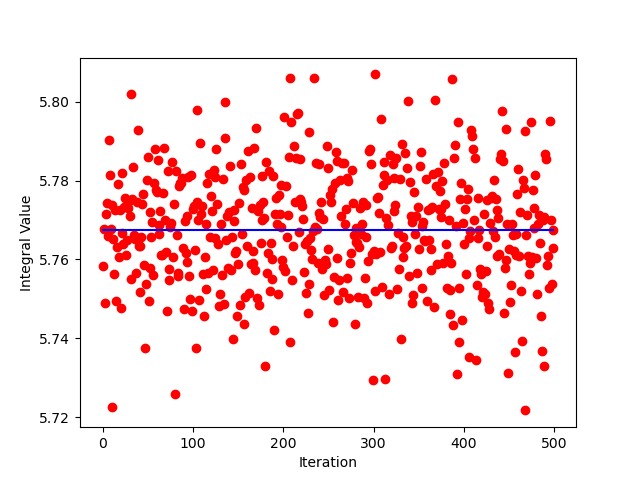
\includegraphics[width=0.4\textwidth]{var_mc.png} 
	} 
	~
	\subfigure[拟蒙特卡洛法500次分布]{ 
	  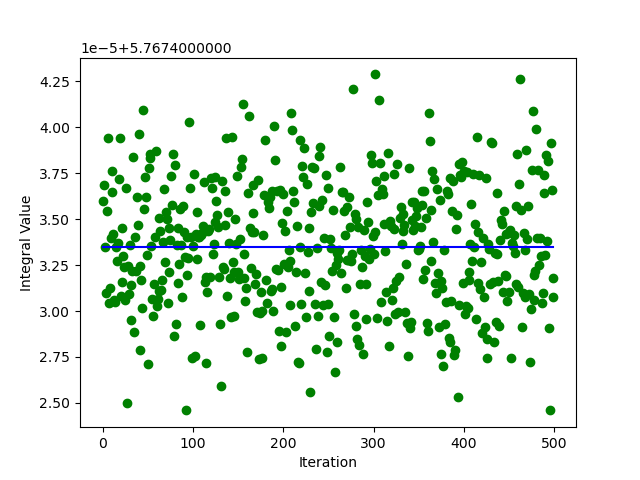
\includegraphics[width=0.4\textwidth]{var_qmc.png} 
	} 
	~ 
	\subfigure[同坐标系显示]{ 
	  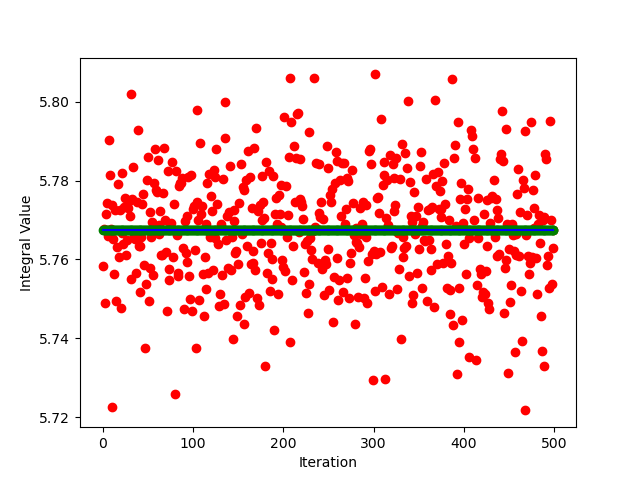
\includegraphics[width=0.4\textwidth]{var_all.png} 
	} 
	\caption{蒙特卡洛和拟蒙特卡罗的分布情况} 
	\label{fig:variance}
\end{figure}

值得一提的是采用拉丁超立方采样的拟蒙特卡洛积分法具有相当小的波动和相当好的准确度,如图~\ref{fig:variance}(c)。和
普通的蒙特卡洛法相比,该方法的分布和真实值相当接近,几乎没有误差。因此这实际上是一个
非常常用的数值积分法。这两类随机方法的均值和方差如表~\ref{tbl:var},拟蒙特卡洛积分法
的方差达到了$10^{-11}$级别,证明了几乎没有显著的波动。


\begin{table}[htbp]
	\centering
	\begin{tabular}{ccc}
		\toprule
		算法 & 均值 & 方差 \\
		\midrule
		蒙特卡洛法 & $5.766607543456825$ & $0.00018877067621830997$ \\
		拟蒙特卡洛法 & $5.767433680428228$ & $1.0746874157286956\times 10^{-11}$ \\
		\bottomrule
	\end{tabular}
	\label{tbl:var}
	\caption{随机方法的均值与方差}
\end{table}

\section{结论}

本次实验实现了龙贝格积分法,并将它与常用的蒙特卡洛法和拟蒙特卡洛法测试和对比,
并简要分析了其中的原因。

龙贝格积分法是一种迭代地逐次提高精度的确定性的方法。它的精度是可以通过提高迭代次数
等方法提高。它迭代提高精度的方式是将误差的一部分补进积分值。经过实验,这种方法在
大多数情况下都有较好的效率,并且在得出确定性结果的同时达到指定精度。

导致龙贝格积分法在某些条件下相对其他两者效率一般的原因可能是因为这个递推过程很难被向量化优化,
尤其是对被积函数求值的过程在时间上的局部性较差。这导致了该实现没有有效利用现代硬件的优化。
但是这造成的性能差异并不显著,并且有可能通过微调算法优化。可见龙贝格积分法是一种非常高效的算法。

尽管在为了达到与蒙特卡洛积分法特别是使用了拉丁超立方采样的拟蒙特卡洛积分法可以比拟的精度,
龙贝格积分法需要较多的迭代次数从而影响了运行效率,但是考虑到拉丁超立方采样在多变量积分
和图形渲染领域的大量应用侧面证明的高效性和准确性,这是正常的。


\clearpage

\appendix

\section{附录:蒙特卡洛积分法和拟蒙特卡洛积分}

使用蒙特卡洛积分是一种采用蒙特卡洛法估计积分的方法。设有积分\eqref{eqn:egint}

\begin{equation}
	\label{eqn:egint}
	I=\int_a^b f(x)d \dif x
\end{equation}

那么可以使用\eqref{eqn:mtest}估计这个积分。其中$pdf(X)$是概率密度函数。特别地
在实现中常取均匀分布$X\sim \mathcal{U}(a,b)$,则$pdf(x)=1/(b-a)$。

\begin{equation}
	\label{eqn:mtest}
	\bar{I_n}=F_n(X)=\frac{1}{n}\sum_{k=1}^n\frac{f(X_k)}{pdf(X_k)}
\end{equation}

\begin{proof}
	要证明这个估计是正确的,就需要证明该估计的数学期望和积分值相等。
\begin{align*}
	E[F_n]&=E\left[\frac{1}{n}\sum_{k=1}^n\frac{f(X_k)}{pdf(X_k)}\right]\\
	&=\frac{1}{n}\sum_{k=1}^n\int \frac{f(x)}{pdf(x)} \cdot pdf(x) \dif x\\
	&=\frac{1}{n}\sum_{k=1}^n\int f(x) \dif x\\
	&=\int f(x) \dif x
\end{align*}
\end{proof}
根据以上结论,可以得到算法~\ref{algo:mcint}

\begin{algorithm}
	\caption{蒙特卡洛法积分}
	\label{algo:mcint}
	\begin{algorithmic}[1]
		\Input{函数$F$,区间$[a,b]$,点数$n$}
		
		\Procedure{Integrate}{$F,a,b,n$}     
		\State $X=[x_1,x_2,x_3,\ldots], x_i \sim\mathcal{U}(a,b)$
		\State $Y=F(X)$
		\State \Return $(b-a)\frac{1}{n}\sum_{i=1}^nY_i$
		\EndProcedure
	\end{algorithmic}
\end{algorithm}	

作为一种随机算法,实际上在$n$较大时有较好的精度,它的收敛速度是$\mathcal{O}(n^{-0.5})$
如果采用\emph{低差异序列}替换纯随机数,积分收敛速度能够达到$\mathcal{O}(n^{-1})$,而且能够避免
随机采样中采样点的聚集。一种简单的一维低差异序列是\emph{Van Der Corput序列}。设有$b$进制数
$x=\sum_{k=0}^md_k\cdot b^k$,则对应的Van der Corput序列可由\eqref{eqn:vdc}计算。

\begin{equation}
	\label{eqn:vdc}
	g_b(x)=\sum_{k=0}^{m}d_k\cdot b^{-k-1}
\end{equation}
$g_b(x)$满足$g_b(x)\in [0,1]$,因此通过区间映射并替代算法~\ref{algo:mcint}中随机数可以得到
拟蒙特卡洛积分算法。此外,还可以使用Latin Hypercube Sampling(拉丁超立方采样)来替代随机数。

\clearpage

\section{附录:代码}
\label{sec:app_code}

\subsection{龙贝格积分实现}
\begin{lstlisting}[language=Python,numbers=left,style=PythonStyle,label={code:romberg},caption=龙贝格积分实现]
import numpy as np

from typing import Callable


def integrate(f: Callable[[np.float], np.float], a: np.float, b: np.float, epsilon: np.float = 0.001,
              n: int = 32) -> np.float:
    r: np.ndarray = np.zeros((n + 1, n + 1), dtype=float)
    h: np.float = b - a
    r[0, 0] = 0.5 * h * (f(a) + f(b))

    p2: int = 1
    for k in range(1, n + 1):
        h *= 0.5
        p2 *= 2

        r[k, 0] = 0.0
        for i in range(1, p2, 2):
            r[k, 0] += f(a + i * h)
        r[k, 0] *= h
        r[k, 0] += 0.5 * r[k - 1, 0]

        p4 = 1
        for m in range(1, k + 1):
            p4 *= 4
            r[k, m] = r[k, (m - 1)] + (r[k, (m - 1)] - r[k - 1, (m - 1)]) / (p4 - 1)

        if k != 1 and np.abs(r[k, 0] - r[(k - 1), 0]) < epsilon:
            return r[k, 0]

    return r[n, 0]
\end{lstlisting}

\subsection{蒙特卡洛法和拟蒙特卡罗法实现}
\begin{lstlisting}[language=Python,numbers=left,style=PythonStyle,label={code:romberg},caption=龙贝格积分实现]
import numpy as np
from scipy.stats import qmc
	
from typing import Callable
def integrate(f: Callable, a: np.float, b: np.float, n: int = 32) -> np.float:
    x = qmc.scale(qmc.LatinHypercube(d=1).random(n), a, b)
    y = f(x)
    y_mean = np.sum(y) / n
    return (b - a) * y_mean


def integrate(f: Callable, a: np.float, b: np.float, n: int = 32) -> np.float:
    x = np.random.uniform(a, b, n)
    y = f(x)
    y_mean = np.sum(y) / n
    return (b - a) * y_mean

\end{lstlisting}

\begin{lstlisting}[language=Python,numbers=left,style=PythonStyle,label={code:romberg},caption=基准测试代码]
import timeit

import numpy as np

from integral.romberg import integrate as i1
from integral.montecarlo import integrate as i2
from integral.qmc import integrate as i3

import matplotlib.pyplot as plt
from integral.romberg import integrate2


def f(x):
    return np.cos(x)


def f2(x):
    return np.power(15 * np.power(x, 3) + 21 * np.power(x, 2) + 41 * x + 3, 1.0 / 4.0) * np.exp(-0.5 * x)


def test_cov(ff, real, a, b):
    val, iters, vals = integrate2(ff, a, b, 0.0001, 128)

    print(val)
    plt.plot(iters, vals, 'ro-', [0, len(iters)], [real, real], 'b')
    plt.xlabel('Iteration')
    plt.ylabel('Integral Value')
    plt.show()


def test_speed():
    rm = []
    mc = []
    qmc = []

    start = timeit.default_timer()
    for i in range(1, 1000):
        i1(f, 0, np.pi / 2, 0.0001, 128)
    rm.append((timeit.default_timer() - start) / 1000)

    start = timeit.default_timer()
    for i in range(1, 1000):
        i1(f2, 0, 4, 0.0001, 128)
    rm.append((timeit.default_timer() - start) / 1000)

    start = timeit.default_timer()
    for i in range(1, 1000):
        i2(f, 0, np.pi / 2, 8192)
    mc.append((timeit.default_timer() - start) / 1000)

    start = timeit.default_timer()
    for i in range(1, 1000):
        i2(f2, 0, 4, 8192)
    mc.append((timeit.default_timer() - start) / 1000)

    start = timeit.default_timer()
    for i in range(1, 1000):
        i3(f, 0, np.pi / 2, 8192)
    qmc.append((timeit.default_timer() - start) / 1000)

    start = timeit.default_timer()
    for i in range(1, 1000):
        i3(f2, 0, 4, 8192)
    qmc.append((timeit.default_timer() - start) / 1000)

    x = np.arange(2)
    total_width, n = 0.8, 3
    width = total_width / n
    x = x - (total_width - width) / 2

    tick_labels = ["f(x)", "g(x)"]
    plt.bar(x, rm, width=width, label='Romberg')
    plt.bar(x + width, mc, width=width, label='Monte Carlo')
    plt.bar(x + 2 * width, qmc, width=width, label='Quasi-Monte Carlo')
    plt.legend()
    plt.xticks(x + width / 2, tick_labels)
    plt.show()


def test_variance():
    iters = []
    vals1 = []
    vals2 = []
    for i in range(1, 500):
        iters.append(i)
        vals1.append(i2(f2, 0, 4, 8192))
        vals2.append(i3(f2, 0, 4, 8192))

    print(np.mean(np.array(vals1, dtype=float)))
    print(np.var(np.array(vals1, dtype=float)))
    print(np.mean(np.array(vals2, dtype=float)))
    print(np.var(np.array(vals2, dtype=float)))

    real = 5.767433490695931
    plt.plot(iters, vals1, 'ro', iters, vals2, 'go', [0, len(iters)], [real, real], 'b')
    plt.xlabel('Iteration')
    plt.ylabel('Integral Value')
    plt.show()

    plt.plot(iters, vals1, 'ro', [0, len(iters)], [real, real], 'b')
    plt.xlabel('Iteration')
    plt.ylabel('Integral Value')
    plt.show()

    plt.plot(iters, vals2, 'go', [0, len(iters)], [real, real], 'b')
    plt.xlabel('Iteration')
    plt.ylabel('Integral Value')
    plt.show()

test_variance()

start = timeit.default_timer()
for i in range(1, 1000):
    i1(f2, 0, 4, 0.0001, 128)
print(timeit.default_timer() - start)

start = timeit.default_timer()
for i in range(1, 10):
    i2(f, 0, np.pi / 2, 8192)
print(timeit.default_timer() - start)

start = timeit.default_timer()
for i in range(1, 1000):
    i3(f2, 0, 4, 8192)
print(timeit.default_timer() - start)

print(i1(f, 0, np.pi / 2, 0.0001, 128),
      i2(f, 0, np.pi / 2, 16384),
      i3(f, 0, np.pi / 2, 8192))
\end{lstlisting}


\end{spacing}

\end{document}